
\documentclass{article}
\usepackage{graphicx}

\begin{document}
	\begin{titlepage}
		\centering
		\vspace*{\fill}
		\includegraphics[width=0.9\textwidth]{logo.jpg}\par % Reducir el tamaño del logo
		\vspace{0.5cm} % Añadir espacio entre el logo y el título
		{\Huge\bfseries Renacer económico de Cuba: El auge de las MIPYMES\par}
		\vspace{5cm}
		{\Large
			Reinaldo Cánovas Gamón\\
			Yilian Vázquez Martínez\\
			Jennifer Rodríguez Moronta\\
			Amalia González Ortega\par
		}
		\vspace*{\fill}
	\end{titlepage}
	
	\newpage

	
	\tableofcontents
	
	\newpage
	
	\section{Introducción}
	En un intento por enfrentar la difícil crisis económica que ha golpeado a Cuba durante décadas, el gobierno cubano tomó una decisión trascendental en septiembre de 2021: la aprobación de más de 9.000 micro, pequeñas y medianas empresas (MIPYMES) en el país. Esta estrategia, sin precedentes en la historia empresarial cubana, busca desencadenar un nuevo impulso económico a través del fomento del sector privado.
	
	La creación de estas MIPYMES se ha convertido en una tabla de salvación para muchas personas en medio de la crisis que ha afectado a la isla durante años. La falta de empleo, la escasez de productos básicos y la restricción de la actividad económica han sido desafíos persistentes que han requerido soluciones innovadoras y audaces.
	Con ese telón de fondo, el presente informe se propone adentrarse en el estudio de las empresas de Cuba, centrándose en las MIPYMES y su evolución a lo largo del tiempo. A través de una narrativa que destacará las historias de valentía, superación y resiliencia de emprendedores cubanos, se busca comprender cómo estas empresas han surgido como una alternativa viable frente a los obstáculos económicos y cómo han influido en el desarrollo y la transformación del ámbito empresarial cubano.
	
	Desde los primeros pioneros empresariales hasta las nuevas oportunidades y los desafíos a los que se enfrentan actualmente, este informe explorará los momentos clave, las estrategias empresariales adoptadas y los impactos socioeconómicos que estas MIPYMES han tenido en Cuba.
	
	A través de una investigación profunda y un análisis riguroso de los datos disponibles, se espera proporcionar una visión integral del panorama empresarial cubano y arrojar luz sobre los desafíos y oportunidades que enfrentan las MIPYMES en el presente y en el futuro.
	
	Adentrémonos ahora en el fascinante mundo de las empresas cubanas y descubramos cómo han contribuido a forjar un nuevo horizonte económico en la isla.
	\newpage
	
	
	\section{Desarrollo}
Después de la devastadora época del Período Especial en Cuba, marcada por una profunda crisis económica y escasez generalizada, surgió un espíritu de determinación en muchos cubanos. Fue en este contexto de adversidad que las micro, pequeñas y medianas empresas (MIPYMES) fueron consideradas como una buena opción de esperanza y renovación para la economía cubana.

En un país donde la mayoría de las actividades económicas estaban dirigidas por el estado, las MIPYMES representarían un rayo de luz en medio de la oscuridad. Estas empresas, en su mayoría dirigidas por emprendedores locales con visión y determinación, se convertirían en motores de desarrollo económico y social. Abriendo pequeñas tiendas, restaurantes, talleres artesanales y servicios especializados, estas MIPYMES no solo generarían empleo, sino que también ofrecerían una variedad de productos y servicios que  eran escasos o inexistentes en el mercado cubano.

Ante este panorama, se concidera la necesidad de permitir y fomentar la creación de empresas privadas en Cuba, como una forma de diversificar la economía, estimular la innovación y generar oportunidades para el desarrollo sostenible del país. Pues considerando esto, la presencia de empresas privadas podría contribuir significativamente a la recuperación económica y al bienestar social de la población cubana.

Así que pensando en esto, en septiembre de 2021, se autorizó la creación de micro, pequeñas y medianas empresas (MIPYMES) en Cuba, lo que marcó un hito significativo en la historia económica del país. Esta decisión fue el resultado de la importancia de fomentar la iniciativa privada y la innovación empresarial para estimular el crecimiento económico y la generación de empleo.

Un estudio realizado tras una información dada por el Ministerio de Economía y Planificación reveló que la autorización de las MIPYMES tuvo un impacto positivo inmediato en las ventas del comercio minorista en Cuba. Según el estudio, las ventas minoristas experimentaron un incremento significativo desde el primer momento de la implementación de esta medida. Este aumento significativo se atribuyó en gran medida al surgimiento de nuevas MIPYMES que ofrecían una variedad de productos y servicios innovadores que antes no estaban disponibles en el mercado cubano.



\begin{figure}[h]
	\centering
	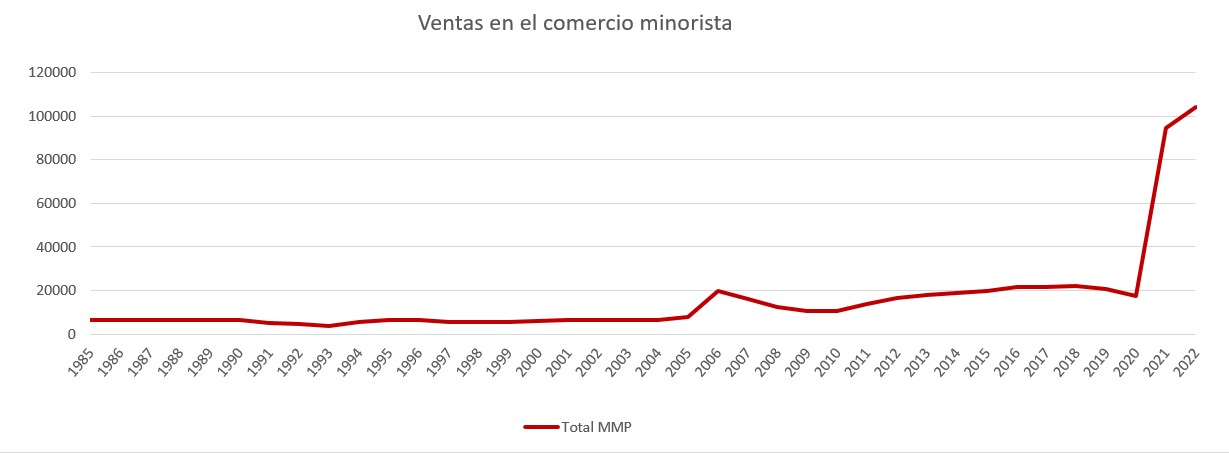
\includegraphics[width=\textwidth]{Ventas.jpg}
	\caption{Muestra del pico de los ingresos en Ventas del comercio minorista en 2021.}
	\label{fig:mi_imagen}
\end{figure}

\newpage

Además, el estudio señaló que las MIPYMES contribuyeron a dinamizar la economía local al generar un mayor flujo de ingresos y empleo, lo que a su vez impulsó el poder adquisitivo de los consumidores. La diversificación de la oferta comercial también atrajo a una mayor cantidad de clientes, lo que resultó en un aumento generalizado de las transacciones comerciales.
Según el informe publicado por el Ministerio de Economía y Planificación, las MIPYMES impactaron significativamente en el aumento de los ingresos en el presupuesto del estado. El estudio reveló que las MIPYMES contribuyeron a dinamizar la economía local al generar un mayor flujo de ingresos y empleo. La diversificación de la oferta comercial también atrajo a una mayor cantidad de clientes, lo que resultó en un aumento generalizado de las transacciones comerciales. Este aumento en la actividad económica ha tenido un impacto directo en el incremento de los ingresos fiscales, lo que ha fortalecido la base impositiva del país y ha contribuido positivamente al presupuesto del estado.


\begin{figure}[h]
	\centering
	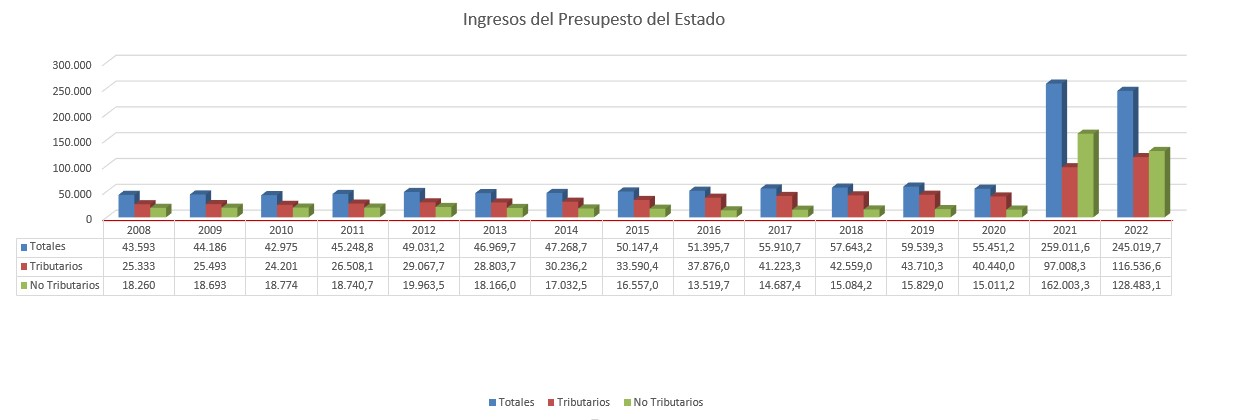
\includegraphics[width=1.0\textwidth]{Ingresos.jpg}
	\caption{Gráfico de los Ingresos en el Presupuesto del Estado .}
	\label{fig:mi_imagen}
\end{figure}


\newpage

El crecimiento exponencial de las MIPYMES desde el 2021 ha sido notable, con un aumento sorprendente que ha llevado a la aparición de más de 9000 empresas en menos de 3 años. Esta tendencia se ha caracterizado por la proliferación de empresas pequeñas, lo que demuestra la importancia que estas entidades han tenido en el panorama empresarial cubano. Este crecimiento ha favorecido los ingresos del presupuesto del estado, aumentando la recaudación fiscal y  fortaleciendo la base impositiva del país.

Una vez aceptadas y reconocidas como parte integral de la economía cubana, las micro, pequeñas y medianas empresas (MIPYMES) han cobrado un protagonismo indiscutible en el panorama empresarial de la isla. Estas empresas, lideradas por emprendedores valientes y visionarios, han demostrado su capacidad para generar empleo, dinamizar la economía local y satisfacer las necesidades del mercado cubano.

Desde su inicio, las MIPYMES, han crecido exponencialmente. Mes tras mes, se ha registrado la creación de más de 300 MIPYMES, lo que ha devenido en un mejor estado del sistema empresarial cubano.


\begin{figure}[h]
	\centering
	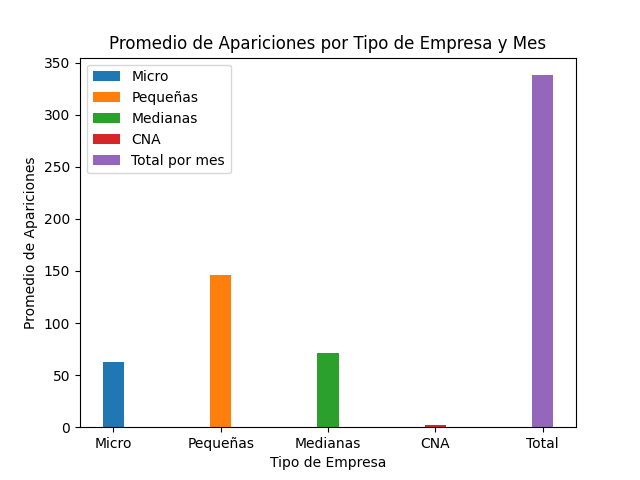
\includegraphics[width=1.0\textwidth]{Apariciones promedio.png}
	\caption{Promedio de las apariciones de las empresas por meses.}
	\label{fig:mi_imagen}
\end{figure}



 De todas las MIPYMES que han surgido, las pequeñas empresas han liderado el camino, superando en número a las empresas micro y medianas. Este fenómeno puede explicarse por varios factores. Por un lado, las pequeñas empresas suelen tener una estructura más sólida y capacidad para ofrecer una gama más amplia de productos y servicios en comparación con las microempresas. Por otro lado, las pequeñas empresas no requieren una inversión tan grande como las medianas, lo que les permite ser más flexibles y adaptables a las condiciones del mercado. El siguiente gráfico visualiza este análisis corroborando que las pequeñas empresas son de preferencia para los emprendedores. 




\begin{figure}[h]
	\centering
	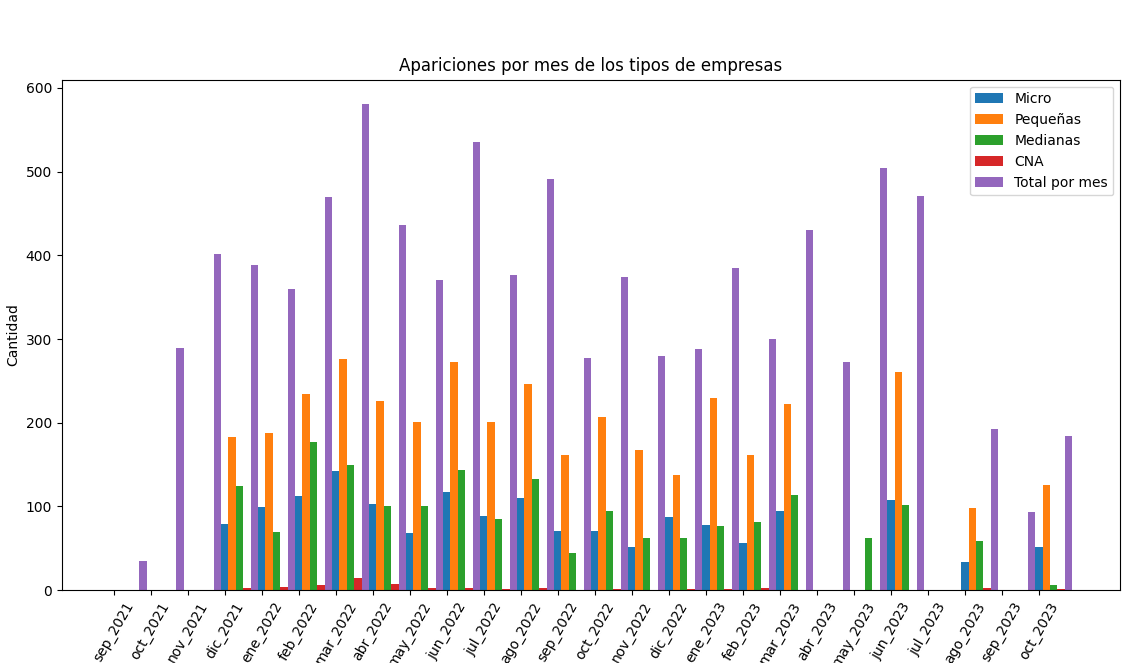
\includegraphics[width=\textwidth]{Figure_3.png}
	\caption{Progreso de las apariciones por meses de las empresas desde 2021.}
	\label{fig:mi_imagen}
\end{figure}



La diversificación de sectores en los que han surgido estas MIPYMES es también un aspecto destacado. Desde pequeñas tiendas de artesanías hasta restaurantes familiares, pasando por servicios especializados en tecnología y reparación de equipos electrónicos, las MIPYMES han demostrado su capacidad para atender una amplia variedad de necesidades del mercado cubano. Esta característica contribuye a enriquecer la oferta de productos y servicios disponibles para los consumidores, promoviendo la competencia y la calidad.

El impacto social de las MIPYMES no puede subestimarse. Estas empresas no solo han generado empleo y MEJORA ECONÓMICA, sino que también han fortalecido el ámbito social al fomentar el espíritu emprendedor y la colaboración entre comunidades. La presencia de MIPYMES ha revitalizado barrios enteros, convirtiéndolos en centros vibrantes de actividad económica y social.

El surgimiento y consolidación de las MIPYMES en Cuba representa un hito importante en la historia económica y social del país. A medida que estas empresas continúan floreciendo, su impacto positivo se hace cada vez más evidente, promoviendo el desarrollo sostenible y ofreciendo esperanza y oportunidades para un futuro próspero en toda la isla.

	\newpage
	
	\section{Conclusiones}
	Las micro, pequeñas y medianas empresas (Mipymes) desempeñan un papel crucial en la economía global, contribuyendo significativamente al crecimiento económico, la generación de empleo y la innovación. Su importancia radica en su capacidad para impulsar el desarrollo sostenible, promover la inclusión social y fomentar la diversificación de la economía. A continuación, se presentan algunas conclusiones sobre la relevancia de las Mipymes en el contexto actual.
	
	En primer lugar, las Mipymes son motores fundamentales del crecimiento económico. A menudo son consideradas como la columna vertebral de muchas economías, ya que representan una gran proporción de las empresas en todo el mundo. Su capacidad para adaptarse rápidamente a los cambios del mercado, así como su agilidad para innovar, les permite impulsar el desarrollo económico a nivel local, regional y nacional.
	
	Además, las Mipymes desempeñan un papel crucial en la generación de empleo. A menudo son los principales empleadores en las comunidades locales, brindando oportunidades laborales a una amplia gama de trabajadores. Esto es especialmente relevante en contextos donde el desempleo es un desafío significativo, ya que las Mipymes pueden contribuir a la reducción de la tasa de desocupación y a la mejora del bienestar de la población.
	
	Asimismo, las Mipymes fomentan la innovación y la diversificación económica. Al ser más ágiles y flexibles que las grandes corporaciones, estas empresas suelen ser incubadoras de nuevas ideas y tecnologías. Además, al operar en sectores diversos y emergentes, contribuyen a la diversificación de la economía, reduciendo la dependencia de un solo sector o industria.
	
	Por otro lado, las Mipymes promueven la inclusión social al brindar oportunidades a segmentos de la población que a menudo enfrentan barreras para acceder al empleo formal. Estas empresas suelen contratar a jóvenes, mujeres, personas con discapacidad y otros grupos marginados, lo que contribuye a la reducción de las desigualdades y a la construcción de sociedades más equitativas.
	
	En resumen, las Mipymes son actores fundamentales en el desarrollo económico y social. Su importancia radica en su capacidad para impulsar el crecimiento, generar empleo, fomentar la innovación, diversificar la economía y promover la inclusión social. Por lo tanto, es crucial que se promueva un entorno propicio para su establecimiento y crecimiento, mediante políticas públicas que faciliten su acceso a financiamiento, tecnología y mercados, así como programas de capacitación y apoyo empresarial. De esta manera, se podrá potenciar el impacto positivo de las Mipymes en las economías locales y globales.
	
	
\end{document}
